\documentclass[a4paper,oneside]{memoir}


\usepackage[T2A]{fontenc} % Поддержка русских букв
\usepackage[utf8]{inputenc} % Кодировка utf8
\usepackage[english,russian]{babel}

\usepackage{lipsum}
\usepackage{graphicx} % Required for including pictures

\usepackage{hyperref}
\usepackage{indentfirst}
\usepackage{amsmath}
\usepackage{amssymb}
\usepackage{amsfonts}
\usepackage{float} 
\usepackage{wrapfig}

%\linespread{1.5} % Line spacing

\title{Курс: "Комбинаторика для начинающих".
	
Неделя 1. Контрольная работа.
	 
Правила сложения и умножения. Принцип Дирихле.}

\newtheorem{task}{Задание}
\newtheorem{solution}{Решение}

 
\author{Александров Алексей, ИУ8-g4}

\date{2020г.}

\begin{document}
	
\maketitle

\begin{task}
	Автомобильные номера штата Калифорнии состоят из одной цифры, не равной 0, трёх больших букв латинского алфавита и ещё трёх цифр (например, 5PPP064). Сколько всего имеется номеров такого типа?
\end{task}

\textbf{Ответ:} $ 9 \cdot 10^{3} \cdot 26^{3} $

\begin{solution}
В качестве первой цифры номера можно взять любую из 9 цифр ($ {1,…,9} $), в качестве каждой из трех букв можно взять любую из 26 букв латинского алфавита, и ещё три цифры, для каждой из которой есть 10 вариантов выбора ({0,…,9}). Итого, по правилу умножения получаем: $ 9 \cdot 10^3 \cdot 26^3 = 158184000 $
\end{solution}

\hrulefill

\begin{task}
Путешественнику нужно добраться из города A в город F двигаясь каждый раз вправо или вверх по стрелкам (см. карту). Сколькими способами это можно сделать?

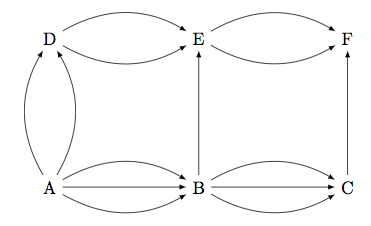
\includegraphics[scale=0.5]{src/roads}

\end{task}

\textbf{Ответ:} $ 23 $

\begin{solution}
	Используя правила сложения и умножения, получаем, что количество способов попасть из $A$ в $F$ равно сумме количества способов пройти по маршрутам $A \rightarrow D \rightarrow E \rightarrow F$, $A \rightarrow B \rightarrow E \rightarrow F$, $A \rightarrow B \rightarrow C \rightarrow F$. В итоге получаем: $2\cdot2\cdot2 + 3\cdot1\cdot2 + 3\cdot3\cdot1 = 8 + 6 + 9 = 23 $.
\end{solution}

\hrulefill

\begin{task}
	В мешке 50 шаров, отличающихся только цветом: 8 красных, 9 синих, 9 желтых, остальные – поровну черные и белые. Какое наименьшее число шаров надо вынуть из мешка, не видя их, чтобы среди них гарантированно было не менее 7 шаров одного цвета?
\end{task}

\textbf{Ответ:} $ 31 $

\begin{solution}
	Сначала заметим, что черных и белых шаров по $ \dfrac{50 - 8 - 9 - 9}{2} = 12 > 7 $. Если взять всего 30 шаров, то может получиться так, что мы взяли только по 6 шаров каждого цвета. Значит, нужно брать больше 30 шаров. Попробуем вытянуть 31 шар. Тогда по принципу Дирихле, если роль "клеток" играют цвета, а роль "кроликов" вытянутые шары, получаем, что какие бы мы ни вытащили шары, среди них обязательно найдется по крайней мере 7 шаров одного цвета(31=5$\cdot$6+1).
\end{solution}

\hrulefill

\begin{task}
15 футбольных команд (в каждой по 11 человек) летят из Москвы в Санкт-Петербург на соревнования. Какое минимальное количество мест может быть в самолете, чтобы гарантированно нашлась команда, долетевшая в полном составе?
\end{task}

\textbf{Ответ:} $ 151 $

\begin{solution}
Если в самолете будет всего 150 мест, то можно будет посадить в него по 10 человек от каждой из 15 команд, тогда самолет будет заполнен целиком, но в нем не будет ни одной команды в полном составе. Значит, нужен с самолет больше, чем со 150150 местами. Рассмотрим самолет, в котором 151 место. Тогда по принципу Дирихле, если роль "клеток" играют команды, а роль "кроликов" футболисты, получаем, что как бы ни произошла рассадка футболистов, среди пассажиров самолета обязательно найдется хотя бы одна команда, летевшая в полном составе (151 = 15 $ \cdot $ 10 + 1).
\end{solution}

\hrulefill

\begin{task}
	Сколько чисел от 1 до 9999 (включая 1 и 9999) не имеют в своей десятичной записи одинаковых подряд идущих цифр? (к примеру, не подходят 1488, 2259, 3233)
\end{task}

\textbf{Ответ:} $ 7380 $

\begin{solution}
Первой цифрой числа, не имеющего в своей записи подряд идущих цифр, может быть любая цифра, кроме 0, то есть всего 9 вариантов.

Второй цифрой этого числа может быть любая цифра, кроме той, которая стоит на первом месте, то есть 9 вариантов, третьей - любая, кроме стоящей на втором месте, то есть опять 9 вариантов, и т.д. Тогда таких четырехзначных чисел всего $ 9^4 $.

Аналогично, трехзначных -- $ 9^3 $

двузначных -- $ 9^2 $

и однозначных -- 9.

Всего получаем: $ 9^4 + 9^3 + 9^2 + 9 = 73809 $ чисел.
\end{solution}

\hrulefill

\begin{task}
	У вас есть 4 ящика и 15 кроликов. Отметьте верные утверждения.
\end{task}

\begin{solution}
При такой рассадке найдётся ящик, в котором сидит $ \geq [\frac{15}{4}] $ кроликов, то есть 4 кролика. Для 5 и 6 кроликов есть контр-пример: $ 4,4,4,3 $.
\end{solution}

\hrulefill

\begin{task}
	Имеется 4 банки желтой краски, 5 банок синей краски и 7 банок красной краски, все банки разного размера. Отметьте верные утверждения.
\end{task}

\begin{solution}
Одну банку краски по правилу сложения можно выбрать $ 4+5+7=16 $ способами. Если же выбирать по одной банке каждой краски, то по правилу умножения получаем  $4 \cdot 5 \cdot 7 = 140$ способов.
\end{solution}

\hrulefill

\end{document}